%%%%%%%%%%%%%%%%%%%%%%%%%%%%%%%%%%%%%%%%%%%%%%%%%%
%
%  This chapter is now in good condition
%
%%%%%%%%%%%%%%%%%%%%%%%%%%%%%%%%%%%%%%%%%%%%%%%%%%


%%%%%%%%%%%%%%%%%%%%%%%%%%%%%%%%%%%%%%%%%%%%%%%%%%%%%%
\chapter{Hatree-Fock Theory}\label{HFT}
\section{The Derivation of Hatree-Fock Theory}
Hatree-Fock theory, can be viewed as the real starting point of
quantum chemistry. The core physical essence of Hatree-Fock theory,
is the single electron approximation. On base of this approximation,
the chemists produce the very common and fundamental chemical
picture so widely used in chemistry: \textbf{the molecular orbitals
and the electrons reside on them.}

\begin{figure}[!hbp]
\begin{center}
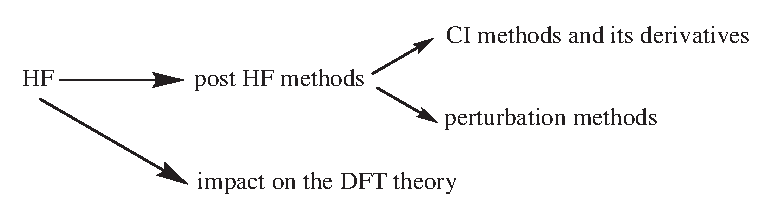
\includegraphics[scale=1.0]{HFpicture.eps}\label{HFT:2}
\caption{description of relationship between HF and other theories}
\end{center}
\end{figure}


%%%%%%%%%%%%%%%%%%%%%%%%%%%%%%%%%%%%%%%%%%%%%%%%%%%%%%%%
\section{Expression of Total Energy}
%
% 1  single electron approximation
% 2  expression of the whole wave function on the base of single electron approximation
% 3  one electron integral
% 4  two electron integral
% 5  the total energy
% 6  the total energy expression based on the basis sets
%
%
%
Here in this chapter, we are going to derive the Hatree-Fock theory.
The way we derive for this section and sections below in this
chapter is taken from some classic quantum chemistry  books
\cite{levine, szabo, pople, dewar}. And the best book to penetrate
into this area, the author recommends the book by Szabo and
Ostlund\cite{szabo}. Herein this section, we designate the $\varphi$
as the molecule orbital, and the $\phi$ as the atomic orbital or
basis sets; the $\Psi$ is used to express the Slater determinant, 
and finally the $\Phi$ is used to denote the wave function based 
on the Slater determinants. Usually the label of $a,b,c,\cdots i,j,k$ etc.
expresses the MO and the Greek letter $\mu, \nu$ etc. signal the AO.
In the following chapter, we will focus on this nomenclature.

The first approximation introduced into the HF theory is the single
electron approximation. For a arbitrary $\Psi$, we suggest that it
contains $n$ electrons; then the introduction of the single electron
approximation means that the $\Psi$ can be decomposed into many
pieces, each is resided by one electron (here we do not involve the
spin into consideration for simplicity); and more importantly, these
piece are not interact with each other. So the $\Psi$ can be written
as:
\begin{equation}\label{}
    \Psi =
    \varphi_{1}(1)\varphi_{2}(2)\varphi_{3}(3)\cdots\varphi_{n}(n)
\end{equation}
This expression is originally promoted by Hatree, which has a
deficiency that it does not incorporate the Pauli restriction to the
wave function. So here the wave function of $\Psi$ is just like the
wave systems we deal with in the classic mechanics. Here, the core
of the single electron approximation, is to simplify the total wave
function containing $n$ electrons into some pieces.

Later slater use the determinant to include the Pauli restriction to
the wave function, and rewrite the $\Psi$ as:
\begin{equation}\label{HFTeq:20}
\Psi = \frac{1}{\sqrt[2]{n!}} \left | \begin{array}{cccc}
  \varphi_{1}(1) & \varphi_{2}(1) & \cdots & \varphi_{n}(1) \\
  \varphi_{1}(2) & \varphi_{2}(2) & \cdots & \varphi_{n}(2) \\
  \cdots & \cdots & \cdots & \cdots                        \\
  \varphi_{1}(n) & \varphi_{2}(n) & \cdots & \varphi_{n}(n)
\end{array} \right |
\end{equation}
So interchanging the $\varphi$ or electron label will lead to the
$\Psi$ to alter its sign. When use the slater determinant form, it's
always appropriate to rewrite it into another equivalent form:
\begin{equation}\label{}
    \Psi = \frac{1}{\sqrt[2]{n!}} \sum_{p}(-1)^{p}P
    \{\varphi_{1}(1)\varphi_{2}(2)\varphi_{3}(3)\cdots\varphi_{n}(n)\}
\end{equation}
Herein this expression, the $P$ is the permutation of the electrons,
which makes electron i permutate over all orbitals. Since there must
be $n!$ terms in the slater determinant, so that we have to multiply
a normalizing factor of $\frac{1}{\sqrt[2]{n!}}$.

So far let's consider the decomposition of the schrodinger operator
of $\hat{H}$:
\begin{equation}\label{HFTeq:21}
    \hat{H}= \left\{\sum_{i=1}^{n}(\frac{-1}{2}\nabla_{i}^2)
    +\sum_{i=1}^{n}\sum_{\alpha=1}^{N}(\frac{-1}{r_{i\alpha}})
    +\sum_{i<j}(\frac{1}{r_{ij}})
\right\}
\end{equation}
It can be divided into two groups, one is the single electron
operator $\hat{H_{1}}$, and the other is the double electron
$\hat{H_{2}}$ operator. $\hat{H_{1}}$ embodies the kinetics and
electron-nuclear operator; and the $\hat{H_{2}}$ embodies the
electron repulsion operator. So let's concentrate on the energy of
each part.

For the $\hat{H_{1}}$, the energy can be expressed as:
\begin{multline}\label{HFTeq:4}
E_{1}=\frac{1}{n!}\langle\Psi|\hat{H_{1}}|\Psi\rangle \\
\shoveleft{=\frac{1}{n!}\sum_{p}\sum_{p^{'}} \langle (-1)^{p}P
\left \{ \varphi_{1}(1)\varphi_{2}(2)\varphi_{3}(3)\cdots\varphi_{n}(n)\right \} |}  \\
\hat{H_{1}}|(-1)^{p^{'}}P^{'} \left \{
\varphi_{1}(1)\varphi_{2}(2)\varphi_{3}(3)\cdots\varphi_{n}(n)\right
\} \rangle
\end{multline}
We can extend $\hat{H_{1}}$here to the form:
\begin{eqnarray}
% \nonumber to remove numbering (before each equation)
  \hat{H_{1}} &=&  \sum_{i=1}^{n}\hat{H}_{single} \nonumber \\
   &=& \sum_{i=1}^{n}\left\{(\frac{-1}{2}\times\nabla_{i}^2)+
   \sum_{\alpha=1}^{N}(\frac{-1}{r_{i\alpha}})\right\}
\end{eqnarray}
So $\hat{H}_{single}$ means the operator on the single electron who
has label of i.

By this way, the integrals of the system orbitals in the
(\ref{HFTeq:4}) can be expressed simply as:
\begin{eqnarray}\label{HFTeq:3}
% \nonumber to remove numbering (before each equation)
 \langle\Psi|\hat{H_{1}}|\Psi\rangle &=& \sum_{i=1}^{n}
\langle\Psi|\hat{H}_{single}|\Psi\rangle \nonumber \\
   &=& n\langle\Psi|\hat{H}_{single}|\Psi\rangle
\end{eqnarray}
For all the n electrons are undistinguished with each other.

So now we can safely assume that the $\hat{H}_{single}$ is the
$\hat{H}(1)$, which means that the operator is from the electron who
has the label of 1.

Moreover, let's interpret the permutation operator in much detailed
form. Since the $\Psi$ is a determinant, the $\Psi$ can be expressed
into the form below according to the Laplace theorem:
\begin{equation}\label{HFTeq:13}
\Psi = \sum^{n}_{i}\varphi_{i}(1)\Delta^{(i,1)}(2,3,4,\cdots,n)
\end{equation}
this expression has a very clear meaning. the $\Delta^{(i,1)}$
represents that the permutation operator is over all the orbitals
and electrons except orbital i and electron 1. this form is
equivalent to the form below:
\begin{equation}
\Psi = \sum^{n}_{i}\varphi_{i}(1) \times (-1)^{i+1} \left |
\begin{array}{cccccc}
  \varphi_{1}(2) & \cdots & \varphi_{i}(2) & \varphi_{i+1}(2) & \cdots & \varphi_{n}(2) \\
  \varphi_{1}(3) & \cdots & \varphi_{i}(3) & \varphi_{i+1}(3) & \cdots & \varphi_{n}(3) \\
  \cdots         & \cdots & \cdots         & \cdots           & \cdots & \cdots         \\
  \varphi_{1}(n) & \cdots & \varphi_{i}(n) & \varphi_{i+1}(n) & \cdots & \varphi_{n}(n)
\end{array}
\right |
\end{equation}
So with (\ref{HFTeq:13}) the (\ref{HFTeq:3}) can be further improved
as:
\begin{multline}\label{}
 \langle\Psi|\hat{H}_{1}|\Psi\rangle =n  \langle
\sum^{n}_{i}\varphi_{i}(1)\Delta^{(i,1)}(2,3,4,\cdots,n) |\\
\hat{H}(1)| \sum^{n}_{j}\varphi_{j}(1)\Delta^{(j,1)}(2,3,4,\cdots,n)
 \rangle
\end{multline}
and it yields:
\begin{multline}\label{HFTeq:14}
\langle\Psi|\hat{H}_{1}|\Psi\rangle = n \langle
\sum^{n}_{i}\varphi_{i}(1)|\hat{H}(1)|
\sum^{n}_{j}\varphi_{j}(1)  \rangle \\
\times \langle \Delta^{(i,1)}(2,3,4,\cdots,n)
|\Delta^{(j,1)}(2,3,4,\cdots,n)
 \rangle
\end{multline}
the $\langle \Delta^{(i,1)}(2,3,4,\cdots,n)
|\Delta^{(j,1)}(2,3,4,\cdots,n)
 \rangle$, is clearly to be $(n-1)!\delta_{ij}$. So with this consideration, it's easily
turned out that only $P=P^{'}$ leads to the
$\langle\Psi|\hat{H}_{1}|\Psi\rangle$ not equal to zero; which means
that the permutation between bra and ket should be same. Upon this
analysis, the (\ref{HFTeq:4}) can be:
\begin{eqnarray}
% \nonumber to remove numbering (before each equation)
  E_{1} &=& \frac{1}{n!}\times n! \langle
\sum^{n}_{i}\varphi_{i}(1)|\hat{H}(1)| \sum^{n}_{j}\varphi_{j}(1)
\rangle \nonumber  \\
   &=&
\sum^{n}_{i}\langle\varphi_{i}(1)|\hat{H}(1)|\varphi_{i}(1) \rangle
\end{eqnarray}
Since the $i$ and $j$ should vary consistently.

The derivation of the double electrons operator is similar to the
derivation for the single electron case above.
\begin{align}\label{}
\hat{H}_{2} &= \sum_{i<j}(\frac{1}{r_{ij}}) \nonumber \\
&=C^{2}_{n}(\frac{1}{r_{12}}) \nonumber \\
&=C^{2}_{n}\hat{H}_{double}
\end{align}
Here because electrons can not distinguish with each other,
therefore we can pick up the electron $1$ and $2$ to represent the
whole double electron operator.

then the energy expectation for the double electron operator is:
\begin{multline}\label{HFTeq:15}
  E_{2}=\frac{1}{n!}\langle\Psi|\hat{H}_{2}|\Psi\rangle \\
  \shoveleft{=\frac{1}{n!}C^{2}_{n}\sum_{p}\sum_{p^{'}}
  \langle
  (-1)^{p} \left \{\varphi_{1}(1)\varphi_{2}(2)\varphi_{3}(3)\cdots\varphi_{n}(n)\right\} |} \\
  \frac{1}{r_{12}}|
  (-1)^{p^{'}}P^{'}
           \left\{\varphi_{1}(1)\varphi_{2}(2)\varphi_{3}(3)\cdots\varphi_{n}(n)\right\}
\rangle
\end{multline}

Similarly, we can express the $\Psi$ as:
\begin{equation}\label{HFTeq:16}
\Psi = \sum^{n}_{i<j}\left|
                       \begin{array}{cc}
                         \varphi_{i}(1) & \varphi_{j}(1) \\
                         \varphi_{i}(2) & \varphi_{j}(2) \\
                       \end{array}
                     \right|
\Delta^{
            i,\,1 \choose
            j,\,2 }
(3,4,\cdots,n)
\end{equation}

By the same procedure used in $\hat{H}_{1}$, the (\ref{HFTeq:15})
can be transformed into the expression below while taking into the
account of (\ref{HFTeq:16}):
\begin{multline}\label{HFTeq:17}
 E_{2}=\frac{1}{n!}C^{2}_{n} \left
 \langle
\Delta^{
            i,\,1 \choose
            j,\,2 }
(3,4,\cdots,n) |
\Delta^{
            k,\,1 \choose
            l,\,2 }
(3,4,\cdots,n) \right\rangle  \\
\left\langle \sum^{n}_{i<j}
 \left|
 \begin{array}{cc}
 \varphi_{i}(1) & \varphi_{j}(1) \\
 \varphi_{i}(2) & \varphi_{j}(2) \\
 \end{array} \right|
 \left |\frac{1}{r_{12}} \right|
 \sum^{n}_{k<l}
  \left|
 \begin{array}{cc}
 \varphi_{k}(1) & \varphi_{l}(1) \\
 \varphi_{k}(2) & \varphi_{l}(2) \\
 \end{array}
 \right|
 \right\rangle
\end{multline}

So let's pay more attention to the (\ref{HFTeq:17}). The expression
below:
\begin{equation}\label{}
\left
 \langle
\Delta^{
            i,\,1 \choose
            j,\,2 }
(3,4,\cdots,n) | \Delta^{
            k,\,1 \choose
            l,\,2 }
(3,4,\cdots,n) \right\rangle
\end{equation}
equals to $(n-2)!\delta_{ik}\delta_{jl}$ (actually we have the
relation that $(i, j) = (k, l)$. However, since the relation that
$i< j$ and $k < l$, $i$ must equal to $k$ and $j$ must equal to $l$
). Thus the integral related to $\frac{1}{r_{12}}$ can be expanded as:
\begin{align}\label{HFTeq:22}
&\delta_{ik}\delta_{jl}\left\langle \sum^{n}_{i<j}
 \left|
 \begin{array}{cc}
 \varphi_{i}(1) & \varphi_{j}(1) \\
 \varphi_{i}(2) & \varphi_{j}(2) \\
 \end{array} \right|
 \left |\frac{1}{r_{12}} \right|
 \sum^{n}_{k<l}
  \left|
 \begin{array}{cc}
 \varphi_{k}(1) & \varphi_{l}(1) \\
 \varphi_{k}(2) & \varphi_{l}(2) \\
 \end{array}
 \right|
 \right\rangle \nonumber \\ 
&=\sum_{i<j}^{n} \left \{
2\langle\varphi_{i}(1)\varphi_{j}(2)|\frac{1}{r_{12}}|
\varphi_{i}(1)\varphi_{j}(2)\rangle -
2\langle\varphi_{i}(1)\varphi_{j}(2)|\frac{1}{r_{12}}|
\varphi_{i}(2)\varphi_{j}(1)\rangle
 \right \}
\end{align}
Since $2\sum_{i<j}$ equals to $\sum_{i}\sum_{j}$ (here we take
notice of the case where $i=j$. In this case (\ref{HFTeq:22}) equal
to $0$), so finally the (\ref{HFTeq:17}) is:
\begin{equation}\label{}
E_{2}=\frac{1}{2}\sum_{i,j}\left\{
\langle\varphi_{i}(1)\varphi_{j}(2)|\frac{1}{r_{12}}|\varphi_{i}(1)\varphi_{j}(2)\rangle-
\langle\varphi_{i}(1)\varphi_{j}(2)|\frac{1}{r_{12}}|\varphi_{j}(1)\varphi_{i}(2)\rangle
\right\}
\end{equation}

All in all,  the total energy is:
\begin{multline}\label{HFTeq:6}
% \nonumber to remove numbering (before each equation)
  E = E_{1}+E_{2}  \\
    \shoveleft{=\sum_{i}^{n}\langle\varphi_{i}(1)|\hat{H}(1)|\varphi_{i}(1)\rangle
    +}  \\
\frac{1}{2}\sum_{i}\sum_{j} \left\{
\langle\varphi_{i}(1)\varphi_{j}(2)|\frac{1}{r_{12}}|\varphi_{i}(1)\varphi_{j}(2)\rangle-
\langle\varphi_{i}(1)\varphi_{j}(2)|\frac{1}{r_{12}}|\varphi_{j}(1)\varphi_{i}(2)\rangle
\right\}
\end{multline}

%%%%%%%%%%%%%%%%%%%%%%%%%%%%%%%%%%%%%%%%%%%%%%%%%%%%%%
\section{General Notion}\label{General_Notion_Hatree-Fock}
%
%
%
%
So far the energy expression has been growing to be very
complicated, so it's appropriate to generalize some notations to
compact the one and two electron integrals.

For the one electron integral:
\begin{equation}\label{HFTeq:28}
\int \varphi^{*}_{i}(1)\hat{H}(1)\varphi_{j}(1) d\tau_{1}
\end{equation}
it's usually shorten as $\langle i|h|j \rangle$, or $[ i|h|j ]$,
$(i|h|j)$ (chemists always use this form), or even $h_{ij}$.

For the two electron integral:
\begin{equation}\label{HFTeq:29}
\int
\varphi^{*}_{i}(1)\varphi^{*}_{j}(2)\frac{1}{r_{12}}\varphi_{k}(1)\varphi_{l}(2)
d\tau_{1} d\tau_{2}
\end{equation}
We usually have two options:
\begin{itemize}
 \item the first option is that we specify it as $\langle ij|kl \rangle$, that
is to put the bra and ket separately. Physicists prefer this expression.
 \item the other option is to express it as $[ ik|jl ]$ or $(ik|jl)$, which we
put the electrons with same label together (ket is followed by bra). This is
favored by chemists.
\end{itemize}

So the (\ref{HFTeq:6}) can be:
\begin{equation}\label{HFTeq:24}
E = \sum^{n}_{i} \langle i|h|i \rangle +
\frac{1}{2}\sum^{n}_{i}\sum^{n}_{j} \{\langle ij|ij \rangle -\langle
ij|ji \rangle \}
\end{equation}
or in the chemical way:
\begin{equation}\label{HFTeq:24-1}
E = \sum^{n}_{i} ( i|h|i ) +
\frac{1}{2}\sum^{n}_{i}\sum^{n}_{j} \{( ii|jj ) -(
ij|ji ) \}
\end{equation}

Usually the differential form of Hatree-Fock equation is difficult
to solve, so that we use the basis sets to expand the molecular
orbitals:
\begin{equation}\label{HFTeq:8}
    \varphi_{i} = \sum_{\mu}c_{\mu i}\phi_{\mu}
\end{equation}
Here the Greek letter indicates the use of the atomic orbitals (AO). By
inserting the expression of $\varphi$ into the
(\ref{HFTeq:6}), we can get:
\begin{multline}\label{HFTeq:7}
E = \sum_{i}\sum_{\mu} \sum_{\nu} C^{*}_{\mu i} C_{\nu
i} \langle\phi_{\mu}(1)|\hat{H}(1)|\phi_{\nu}(1)\rangle +  \\
\frac{1}{2} \sum_{i}\sum_{j}\sum_{\mu} \sum_{\nu} \sum_{\lambda}
\sum_{\sigma} C^{*}_{\mu i} C_{\nu i} C^{*}_{\lambda j} C_{\sigma j}
\\
 \left\{
\langle\phi_{\mu}(1)\phi_{\lambda}(2)|\hat{H}(12)|\phi_{\nu}(1)\phi_{\sigma}(2)\rangle-
\langle\phi_{\mu}(1)\phi_{\lambda}(2)|\hat{H}(12)|\phi_{\sigma}(1)\phi_{\nu}(2)\rangle
\right \}
\end{multline}
Here according to the notation we have discussed, we can make some
abbreviations to the (\ref{HFTeq:7}), to make it looks more clear.
First, we can abbreviate the single electron integral as:
\begin{equation}\label{}
\langle\phi_{\mu}|\hat{H}(1)|\phi_{\nu}\rangle = h_{\mu \nu}
\end{equation}
Then the double electron integral can be written as:
\begin{equation}\label{}
% \nonumber to remove numbering (before each equation)
  \langle\phi_{\mu}(1)\phi_{\lambda}(2)|\hat{H}(12)|\phi_{\nu}(1)\phi_{\sigma}(2)\rangle
  = \langle \mu\lambda | \nu\sigma \rangle
\end{equation}
Furthermore, we can define the ``density matrix'' as
$\sum_{i}C^{*}_{\mu i} C_{\nu i} = P_{\mu\nu}$. whose meaning
will be further discussed in the following content.

On the base of the discussion above, we have (\ref{HFTeq:7}) shorten
as:
\begin{equation}\label{HFTeq:11}
    E = \sum_{\mu \nu}P_{\mu\nu}h_{\mu \nu} + \frac{1}{2}
    \sum_{\mu \nu \lambda\sigma}P_{\mu\nu}P_{\lambda\sigma}
    \left \{ \langle\mu\lambda | \nu\sigma\rangle - \langle\mu \lambda | \sigma\nu\rangle
    \right \}
\end{equation}
Or the form that:
\begin{equation}\label{HFTeq:11-1}
    E = \sum_{\mu \nu}P_{\mu\nu}h_{\mu \nu} + \frac{1}{2}
    \sum_{\mu \nu \lambda\sigma}P_{\mu\nu}P_{\lambda\sigma}
    \left \{ (\mu\nu|\lambda\sigma) - (\mu \sigma|\lambda\nu)
    \right \}
\end{equation}

%%%%%%%%%%%%%%%%%%%%%%%%%%%%%%%%%%%%%%%%%%%%%%%%%%%

\section{Physical Meaning of Total Energy}\label{PMTE_for_HF}
% the most important concept is orbitals are independent with each other,
% so there's no cross terms in the energy expression
% one electron integral: no cross terms
% coulomb energy, how to count
% exchange energy, how to count; the origin is from determinant
% on the basis sets, how to understand the density
% how to understand the density matrix
%
Here we can see what's the meaning of the total energy. And now
let's interpret it in a more pictorial way.

The essence of HF theory, is to approximate the wave function as
slater determinant. Since the orbitals are not interact with each
other, it can be well expected that there's no cross term in the
energy expression; and the derivation above indeed demonstrates this
point.

The one electron integral, is divided into two parts: the electron
kinetic energy and nuclear electron attraction energy. From the last
section it can see that their expectation values are summing over
all orbitals, and no cross term in the final result.

As for the double electron integral, it can be partitioned into two
parts: the coulomb energy and the exchange energy. Before we step
into the physical interpretation of both of the two terms, let's
shift to the real picture of the interaction between two electrons.

Suppose that we have electron 1 at place $\tau_{1}$ and electron 2
at place $\tau_{2}$, if there's little change in the motion of
electron 2 will cause instantaneous motion change in electron 1.
This is coincident with the uncertainty law: in quantum mechanical
world, the motion of any two electrons can never be independent with
each other since that their wave functions can be always superposed
together so that the interaction happens.

However, in Hatree-Fock picture the electrons are assumed to be
independent with each other, thus there must be some part of effects
which fail to conclude into the energy expression, this part is
called correlation energy.

Then let's go to see the coulomb energy. First we can specify the
term in (\ref{HFTeq:6}) as:
\begin{equation}\label{}
\frac{1}{2}\sum_{i}\sum_{j} \int
\varphi^{*}_{i}(1)\varphi_{i}(1)
\frac{1}{r_{12}}\varphi^{*}_{j}(2)\varphi_{j}(2)
d\tau_{1} d\tau_{2}
\end{equation}

Here the $|\varphi_{i}(1)|^{2}d\tau_{1}$ represents the
infinitesimal density of electron 1 at position of $d\tau_{1}$, so
as the $|\varphi_{j}(2)|^{2}d\tau_{2}$; and the integral under
operation of $\frac{1}{r_{12}}$ denotes the coulomb energy between
electron 1 at position of $d\tau_{1}$ and electron 2 at position of
$d\tau_{2}$. By summing up all the $j$ orbitals as well as summing
up over all the $i$ orbitals, we can get the average coulomb
potential felt by the electron density at position 1 and position 2. Finally
since we count each one orbital twice, we times a factor of $1/2$. Hence we can
actually express it into much more clear form:
\begin{align}\label{HF_PMTE_eq:1}
&\frac{1}{2}\sum_{i}\sum_{j} \int
\varphi^{*}_{i}(1)\varphi_{i}(1)
\frac{1}{r_{12}}\varphi^{*}_{j}(2)\varphi_{j}(2)
d\tau_{1} d\tau_{2} \nonumber \\
&= \frac{1}{2} \int \rho(r)
\frac{1}{|r-r^{'}|}\rho(r^{'})
d r dr^{'}
\end{align}

In the coulomb energy expression, it's interesting to see that it's
irrelevant to the spin consideration. therefore, if we assume
there's one electron on the molecular orbital, then we use the
result above; if two electrons occupied on the orbital, then we
multiply a factor of $2$ since both of the two electrons make same
contributions.

The exchange term from the (\ref{HFTeq:6}) is arising from the
antisymmetric nature of the single determinant, and it has a
somewhat strange form and does not have a simple classic
interpretation like coulomb term:
\begin{equation}\label{}
-\frac{1}{2}\sum_{i}\sum_{j} \int \varphi^{*}_{i}(1)\varphi_{j}(1)
\frac{1}{r_{12}}\varphi^{*}_{j}(2)\varphi_{i}(2) d\tau_{1} d\tau_{2}
\end{equation}

However, we can still use some simple notion to express it:
\begin{align}\label{HF_PMTE_eq:2}
& -\frac{1}{2}\sum_{i}\sum_{j} \int \varphi^{*}_{i}(1)\varphi_{j}(1)
\frac{1}{r_{12}}\varphi^{*}_{j}(2)\varphi_{i}(2) d\tau_{1} d\tau_{2} \nonumber
\\
& =  -\frac{1}{2}\sum_{i}\sum_{j} \int \varphi^{*}_{i}(1)\varphi_{i}(2)
\frac{1}{r_{12}}\varphi^{*}_{j}(2)\varphi_{j}(1) d\tau_{1}
d\tau_{2} \rightarrow \nonumber \\
&= -\frac{1}{2}\int \rho(r1, r2)\frac{1}{r_{12}}\rho(r2, r1)d\tau_{1}
d\tau_{2} \rightarrow \nonumber \\
&=  -\frac{1}{2}\int \rho(r, r^{'})\frac{1}{|r-r^{'}|}\rho(r^{'}, r)dr
dr^{'}
\end{align}
Here we introduce the exchange density $\rho(r1, r2) =
\sum_{i}\varphi^{*}_{i}(1)\varphi_{i}(2)$. Physically, this new density relies
on two position index (so it reflects the non-local property of the exchange
energy). In fact, in the following chapter discussing the reduced density
matrix, we can see that this is just the one dimensional reduced density matrix.

Now let's consider spin. It's obvious that $\rho_{\sigma\sigma^{'}}(r, r^{'}) =
0$ if $\sigma \neq \sigma^{'}$. Actually in the density matrix part, we can
show that:
\begin{equation}
 \int \rho_{\sigma\sigma^{'}}(r, r^{'}) dr^{'} = -\delta_{\sigma\sigma^{'}}
\end{equation}
This is called ``Fermi Hole'' for the exchange effects.

Finally let's go to see the density:
\begin{align}\label{HF_PMTE_eq:3}
 \rho(r) &= \sum_{i}|\varphi_{i}(r)|^{2} \nonumber \\
&= \sum_{i}\sum_{\mu}\sum_{\nu}c^{*}_{\mu i}c_{\nu i}\phi^{*}_{\mu}\phi_{\nu}
\nonumber \\
&= \sum_{\mu}\sum_{\nu}P_{\mu\nu}\phi^{*}_{\mu}\phi_{\nu}
\end{align}
It can be further partitioned by two parts:
\begin{align}\label{HF_PMTE_eq:4}
&\sum_{\mu}\sum_{\nu}P_{\mu\nu}\phi^{*}_{\mu}\phi_{\nu} \nonumber \\
&= \sum_{\mu}P_{\mu\nu}|\phi_{\mu}|^{2} + 
2\sum_{\mu<\nu}P_{\mu\nu}\phi^{*}_{\mu}\phi_{\nu}
\end{align}

Here in this expression, the $\sum_{\mu}P_{\mu\nu}|\phi_{\mu}|^{2}$ express the
electron density coming from the $\mu$th atom; and the other part where $\mu
< \nu$ describe the overlap of the orbitals which is coming from
different atoms, that makes up another part of the electron density.
Therefore by translating the abstract molecule orbital into the
concrete basis sets, we can have a more pictorial way to look into
the HF theory.

For the density matrix, who has the form of $\sum_{i}C^{*}_{\mu i}
C_{\nu i} = P_{\mu\nu}$; that is the summation of electron
density of all molecule orbitals, and between $\mu$th atom and
$\nu$th atom. if $\mu=\nu$, that indicates the pure electron distribution
of the atom $\mu$; if $\mu \neq \nu$, this indicates the electron
distribution within the area between atom $\mu$ and $\nu$, which can
be related to the chemical bond between atom $\mu$ and $\nu$.  In the following
section, we will move back to it again.


%%%%%%%%%%%%%%%%%%%%%%%%%%%%%%%%%%%%%%%
\section{Restricted and Unrestricted Cases}\label{RUC_in_HF}
%
%
There are generally two ways to form the Slater determinants: one is
the restricted type and the other is the unrestricted type. In the restricted
type (RHF or ROHF), the electrons in the molecule are grouped into pairs to
reside on the molecular orbitals starting from the lowest energy one; while in
the other case (UHF) the electrons in different spin states are assumed to
independently occupy the orbitals, that means their spatial part is also
different (see \ref{HFTpic:4}). 

\begin{figure}[htbp]
\begin{center}
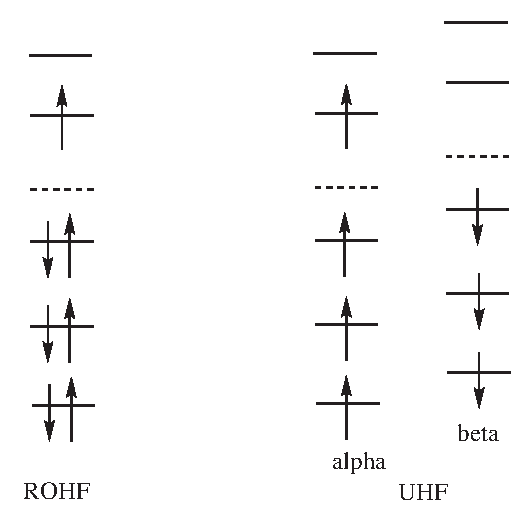
\includegraphics[scale=0.7]{uhfrohf.eps}
\caption{UHF and ROHF description}
\label{HFTpic:4}
\end{center}
\end{figure}

Let's start from our last section conclusion, that to express the terms into
density and exchange density form. For the one electron integral, actually the
spin will not affect its form. For the coulomb part, it's irrelevant to the
density, and for the exchange density, the spin cross term is zero. Hence let's
consider:
\begin{align}\label{}
r(\alpha) \quad &  r^{'}(\alpha) \nonumber \\
r(\alpha) \quad &  r^{'}(\beta) \nonumber \\
r(\beta) \quad &  r^{'}(\alpha) \nonumber \\
r(\beta) \quad &  r^{'}(\beta) \nonumber \\
\end{align}
For the coulomb term, all of four terms exist; and for exchange energy, the
second and third term vanish. Hence we can express the total energy generally
as:
\begin{equation}
  E = h_{\mu\nu}^{\alpha} + h_{\mu\nu}^{\beta} 
   + \frac{1}{2}\left[ C_{\alpha\alpha} + 
C_{\alpha\beta} + C_{\beta\alpha} + C_{\beta\beta}\right] -
\frac{1}{2}\left[ X_{\alpha\alpha} + X_{\beta\beta} \right] 
\end{equation}
Here $C_{\alpha\alpha}$ etc. is the terms expressed in (\ref{HF_PMTE_eq:1}) by
adding the spin consideration, and $X_{\alpha\alpha}$ is the exchange term in 
(\ref{HF_PMTE_eq:2}).

For the RHF case, we can get:
\begin{equation}\label{HFTeq:23}
  E = 2h_{\mu\nu} 
   + \left[ 2C_{r, r^{'}}  -  X_{r, r^{'}}  \right] 
\end{equation}
Since we need not to specify spin state anymore, so we just specify the
position vector.

For the UHF case
\begin{equation}\label{HFTeq:27}
  E = h_{\mu\nu}^{\alpha} + h_{\mu\nu}^{\beta}  
   + \frac{1}{2}\left[ C_{\alpha\alpha} + 
C_{\alpha\beta} + C_{\beta\alpha} + C_{\beta\beta}\right] -
\frac{1}{2}\left[ X_{\alpha\alpha} + X_{\beta\beta} \right] 
\end{equation}
Since alpha part and beta usually not equal to each other anymore.


%%%%%%%%%%%%%%%%%%%%%%%%%%%%%%%%%%%%%%%%%%%%
\section{The Derivation of The Hatree-Fock Equation}
\subsection{Variation Process}\label{HFT:6}
% 1  physical meaning of the variation process: through the variation
%     of total energy we get the HF function
% 2  meaning of HF function
%
%
%
From the discussion above, we can see that under single electron
approximation; the total energy has been expressed as the functional
of orbitals. So eventually, the total energy is the functional of
the molecule orbital space. Under the constraint of maintaining
perpendicular condition (this is required by the single electron
approximation), as the molecule orbitals continuously make an
infinitesimal change, the total energy is also coincidentally
changed. Our target, is to find the expression as $\frac{\delta
E}{\delta \Psi} = 0$. That's the stationary point of the
$E=F[\Psi]$\footnote{Personally I hate this long derivation. However, it's
detailed and rigorous. On the other hand, we need a point of view that to
understand the HF theory from the MO variation}.

The perpendicular condition required in the variation process is:
\begin{align}\label{}
    \int\delta\varphi_{i}\varphi_{j}d\tau &= \delta_{ij} \nonumber \\
    \int\varphi_{i}\delta\varphi_{j}d\tau &= \delta_{ij}
\end{align}
It's worthy to note that in the variational process, we care about the first
order varied $\Psi$ so all the second order terms, like
$\delta\varphi_{i}\delta\varphi_{j}$ are all ignored.

Now we enter the variation process. Under such constraint, it's
necessarily to use the lagrange variation process. Firstly, let's go
into the variation process based on the molecule orbitals.

As molecule orbital
$\varphi_{i}\rightarrow\varphi_{i}+\delta\varphi_{i}$, the energy is
also changed $E\rightarrow E+\delta E$. We vary the expression
below(the general total energy expression is concerned):
\begin{multline}\label{HFTeq:1}
% \nonumber to remove numbering (before each equation)
  G =\sum_{i}^{n}\langle\varphi_{i}(1)|\hat{H}(1)|\varphi_{i}(1)\rangle
    +  \\
\frac{1}{2}\sum_{i}\sum_{j} \left\{
\langle\varphi_{i}(1)\varphi_{j}(2)|\frac{1}{r_{12}}|\varphi_{i}(1)\varphi_{j}(2)\rangle-
\langle\varphi_{i}(1)\varphi_{j}(2)|\frac{1}{r_{12}}|\varphi_{j}(1)\varphi_{i}(2)\rangle
\right\} \\
-(\sum_{i}\sum_{j}\varepsilon_{ij}\langle\varphi_{i}(1)|\varphi_{j}(1)\rangle
-\delta_{ij} )
\end{multline}
The last term introduce the orthogonality restriction in the MO variation
process.

Obviously the G is different from E only by a constant added by the
final term. Here $\varepsilon_{ij}$ is purely some Lagrangian
factor.

Therefore, $\delta G$ gets to:
\begin{multline}\label{HFTeq:2}
\delta G = \sum_{i}^{n} \left \{
\langle\delta\varphi_{i}(1)|\hat{H}(1)|\varphi_{i}(1)\rangle +
\langle\varphi_{i}(1)|\hat{H}(1)|\delta\varphi_{i}(1)\rangle
\right\} +  \\
\frac{1}{2}\sum_{i}\sum_{j} \left\{
\langle\delta\varphi_{i}(1)\varphi_{j}(2)|\frac{1}{r_{12}}|\varphi_{i}(1)\varphi_{j}(2)\rangle
+
\langle\varphi_{i}(1)\delta\varphi_{j}(2)|\frac{1}{r_{12}}|\varphi_{i}(1)\varphi_{j}(2)\rangle
\right\} +  \\
\frac{1}{2}\sum_{i}\sum_{j} \left\{
\langle\varphi_{i}(1)\varphi_{j}(2)|\frac{1}{r_{12}}|\delta\varphi_{i}(1)\varphi_{j}(2)\rangle
+
\langle\varphi_{i}(1)\varphi_{j}(2)|\frac{1}{r_{12}}|\varphi_{i}(1)\delta\varphi_{j}(2)\rangle
\right\} - \\
\frac{1}{2}\sum_{i}\sum_{j} \left\{
\langle\delta\varphi_{i}(1)\varphi_{j}(2)|\frac{1}{r_{12}}|\varphi_{j}(1)\varphi_{i}(2)\rangle
+
\langle\varphi_{i}(1)\delta\varphi_{j}(2)|\frac{1}{r_{12}}|\varphi_{j}(1)\varphi_{i}(2)\rangle
\right\} - \\
\frac{1}{2}\sum_{i}\sum_{j} \left\{
\langle\varphi_{i}(1)\varphi_{j}(2)|\frac{1}{r_{12}}|\delta\varphi_{j}(1)\varphi_{i}(2)\rangle
+
\langle\varphi_{i}(1)\varphi_{j}(2)|\frac{1}{r_{12}}|\varphi_{j}(1)\delta\varphi_{i}(2)\rangle
\right\} \\
- \sum_{i}\sum_{j} \varepsilon_{ij}\left\{
\langle\delta\varphi_{i}(1)|\varphi_{j}(1)\rangle +
\langle\varphi_{i}(1)|\delta\varphi_{j}(1)\rangle
 \right\}
\end{multline}

Now first we have to make some implications for the (\ref{HFTeq:2}).
There's two general rules for us; since that the operator of
$1/r_{12}$ is some hermite operator then we can safely exchange the
bra and ket, that's the first transformation; secondly, because the
electrons are undistinguished with each other thus we can exchange
the electron label in the integrals without changing it.

For the coulomb integrals, let's use the first rule to exchange the
bra and ket; then we can find:
\begin{align}\label{}
\langle\delta\varphi_{i}(1)\varphi_{j}(2)|\frac{1}{r_{12}}|
\varphi_{i}(1)\varphi_{j}(2)\rangle &=
\langle\varphi_{i}(1)\varphi_{j}(2)|\frac{1}{r_{12}}|
\delta\varphi_{i}(1)\varphi_{j}(2)\rangle \nonumber \\
\langle\varphi_{i}(1)\delta\varphi_{j}(2)|\frac{1}{r_{12}}|
\varphi_{i}(1)\varphi_{j}(2)\rangle &=
\langle\varphi_{i}(1)\varphi_{j}(2)|\frac{1}{r_{12}}|
\varphi_{i}(1)\delta\varphi_{j}(2)\rangle
\end{align}

For the exchange integrals, firstly we exchange the electron label
then then do the same thing for the bra and ket; finally we can get:
\begin{align}\label{}
\langle\delta\varphi_{i}(1)\varphi_{j}(2)|\frac{1}{r_{12}}|
\varphi_{j}(1)\varphi_{i}(2)\rangle &=
\langle\varphi_{i}(1)\varphi_{j}(2)|\frac{1}{r_{12}}|
\varphi_{j}(1)\delta\varphi_{i}(2)\rangle \nonumber \\
\langle\varphi_{i}(1)\delta\varphi_{j}(2)|\frac{1}{r_{12}}|
\varphi_{j}(1)\varphi_{i}(2)\rangle &=
\langle\varphi_{i}(1)\varphi_{j}(2)|\frac{1}{r_{12}}|
\delta\varphi_{j}(1)\varphi_{i}(2)\rangle
\end{align}

Finally, by gathering all the results above, we can transform the
(\ref{HFTeq:2}) into:
\begin{multline}\label{}
\delta G = \sum_{i}^{n} \left \{
\langle\delta\varphi_{i}(1)|\hat{H}(1)|\varphi_{i}(1)\rangle +
\langle\varphi_{i}(1)|\hat{H}(1)|\delta\varphi_{i}(1)\rangle
\right\} +  \\
\sum_{i}\sum_{j} \left\{
\langle\delta\varphi_{i}(1)\varphi_{j}(2)|\frac{1}{r_{12}}|\varphi_{i}(1)\varphi_{j}(2)\rangle
+
\langle\varphi_{i}(1)\varphi_{j}(2)|\frac{1}{r_{12}}|\varphi_{i}(1)\delta\varphi_{j}(2)\rangle
\right\} - \\
\sum_{i}\sum_{j} \left\{
\langle\delta\varphi_{i}(1)\varphi_{j}(2)|\frac{1}{r_{12}}|\varphi_{j}(1)\varphi_{i}(2)\rangle
+
\langle\varphi_{i}(1)\varphi_{j}(2)|\frac{1}{r_{12}}|\delta\varphi_{j}(1)\varphi_{i}(2)\rangle
\right\} \\
- \sum_{i}\sum_{j} \varepsilon_{ij}\left\{
\langle\delta\varphi_{i}(1)|\varphi_{j}(1)\rangle +
\langle\varphi_{i}(1)|\delta\varphi_{j}(1)\rangle
 \right\}
\end{multline}
Here for the two electron integrals, we drive all the
$\delta\varphi_{i}$ into the bra, and $\delta\varphi_{j}$ into the
ket.

Furthermore, the above expression can be classified into two groups;
that is:
\begin{equation}\label{HFTeq:33}
\begin{split}
\delta G  &=
\Bigg\{ \sum_{i}^{n}
\langle\delta\varphi_{i}(1)|\hat{H}(1)|\varphi_{i}(1)\rangle
 +
\sum_{i}\sum_{j} \left(
\langle\delta\varphi_{i}(1)\varphi_{j}(2)|\frac{1}{r_{12}}|
\varphi_{i}(1)\varphi_{j}(2)\rangle - \right. \\
&\left.\langle\delta\varphi_{i}(1)\varphi_{j}(2)|\frac{1}{r_{12}}|
\varphi_{j}(1)\varphi_{i}(2)\rangle \right) - \sum_{i}\sum_{j}
\varepsilon_{ij}
\langle\delta\varphi_{i}(1)|\varphi_{j}(1)\rangle \Bigg\} + \\
&\Bigg\{ \sum_{i}^{n}
\langle\varphi_{i}(1)|\hat{H}(1)|\delta\varphi_{i}(1)\rangle
 +
\sum_{i}\sum_{j} \left(
\langle\varphi_{i}(1)\varphi_{j}(2)|\frac{1}{r_{12}}|
\varphi_{i}(1)\delta\varphi_{j}(2)\rangle - \right. \\
&\left.\langle\varphi_{i}(1)\varphi_{j}(2)|\frac{1}{r_{12}}|
\delta\varphi_{j}(1)\varphi_{i}(2)\rangle \right) - \sum_{i}\sum_{j}
\varepsilon_{ij}
\langle\varphi_{i}(1)|\delta\varphi_{j}(1)\rangle\Bigg\}
\end{split}
\end{equation}

Continuously, we can exchange the label of electrons to further
simplify the (\ref{HFTeq:33}). Firstly we have:
\begin{equation}\label{}
\begin{split}
& \langle\varphi_{i}(1)\varphi_{j}(2)|\frac{1}{r_{12}}|
\varphi_{i}(1)\delta\varphi_{j}(2)\rangle -
\langle\varphi_{i}(1)\varphi_{j}(2)|\frac{1}{r_{12}}|
\delta\varphi_{j}(1)\varphi_{i}(2)\rangle \\
&= \langle\varphi_{i}(1)\varphi_{j}(2)|\frac{1}{r_{12}}|
\varphi_{i}(1)\delta\varphi_{j}(2)\rangle -
\langle\varphi_{i}(2)\varphi_{j}(1)|\frac{1}{r_{12}}|
\delta\varphi_{j}(2)\varphi_{i}(1)\rangle
\end{split}
\end{equation}

Then by bringing the above result into the (\ref{HFTeq:33}), we can
have:
\begin{equation}\label{HFTeq:34}
\begin{split}
\delta G  &= \Bigg\{ \sum_{i}^{n}
\langle\delta\varphi_{i}(1)|\hat{H}(1)|\varphi_{i}(1)\rangle
 +
\sum_{i}\sum_{j} \left(
\langle\delta\varphi_{i}(1)\varphi_{j}(2)|\frac{1}{r_{12}}|
\varphi_{i}(1)\varphi_{j}(2)\rangle - \right. \\
&\left.\langle\delta\varphi_{i}(1)\varphi_{j}(2)|\frac{1}{r_{12}}|
\varphi_{j}(1)\varphi_{i}(2)\rangle \right) - \sum_{i}\sum_{j}
\varepsilon_{ij}
\langle\delta\varphi_{i}(1)|\varphi_{j}(1)\rangle \Bigg\} + \\
&\Bigg\{ \sum_{j}^{n}
\langle\varphi_{j}(2)|\hat{H}(2)|\delta\varphi_{j}(2)\rangle
 +
\sum_{i}\sum_{j} \left(
\langle\varphi_{i}(1)\varphi_{j}(2)|\frac{1}{r_{12}}|
\varphi_{i}(1)\delta\varphi_{j}(2)\rangle - \right. \\
&\left.\langle\varphi_{j}(1)\varphi_{i}(2)|\frac{1}{r_{12}}|
\varphi_{i}(1)\delta\varphi_{j}(2)\rangle \right) - \sum_{i}\sum_{j}
\varepsilon_{ij}
\langle\varphi_{i}(2)|\delta\varphi_{j}(2)\rangle\Bigg\}
\end{split}
\end{equation}

Now thing becomes clear. In the (\ref{HFTeq:34}) we note that the
$\langle\delta\varphi_{i}|$ and $|\delta\varphi_{j}\rangle$ vary
independently, thus we can write the (\ref{HFTeq:34}) generally as:
\begin{multline}\label{HFTeq:5}
\delta G = \sum_{i}^{n}
\langle\delta\varphi_{i}(1)|\hat{H}(1)|\varphi_{i}(1)\rangle \\
+ \sum_{i}\sum_{j} \left\{
\langle\delta\varphi_{i}(1)\varphi_{j}(2)|\frac{1}{r_{12}}|\varphi_{i}(1)\varphi_{j}(2)\rangle
-
\langle\delta\varphi_{i}(1)\varphi_{j}(2)|\frac{1}{r_{12}}|\varphi_{j}(1)\varphi_{i}(2)\rangle
\right\} \\
- \sum_{i}\sum_{j} \varepsilon_{ij}
\langle\delta\varphi_{i}(1)|\varphi_{j}(1)\rangle + \text {other
terms}
\end{multline}

Therefore as $\delta G = 0$ then the two independent
$\langle\delta\varphi_{i}|$ and $|\delta\varphi_{j}\rangle$ will
become zero separately, that means each sum will go zero in the
independent way in the (\ref{HFTeq:34}). Then in the (\ref{HFTeq:5})
we can lift the $\sum_{i}^{n}\langle\delta\varphi_{i}(1)|$ outside,
it gives:
\begin{multline}\label{HFTeq:9}
\hat{H}(1)\varphi_{i}(1) + \sum_{j}^{occ}\left[
\left\{\int\varphi^{*}_{j}(2)\varphi_{j}(2)d\tau(2)\frac{1}{r_{12}}\right\}\varphi_{i}(1)
\right] \\
 -
\sum_{j}^{occ}\left[
\left\{\int\varphi^{*}_{j}(2)\varphi_{i}(2)d\tau(2)\frac{1}{r_{12}}\right\}\varphi_{j}(1)
\right] \\
 = \sum_{j} \varepsilon_{ij}\varphi_{j}(1)
\end{multline}
This is the most famous Hatree-Fock Equation.

If we define two new operator related to the coulomb and exchange
term, we can have:
\begin{eqnarray}\label{HFTeq:31}
% \nonumber to remove numbering (before each equation)
  J_{i} &=& \int\varphi^{*}_{j}(2)\varphi_{j}(2)d\tau(2)\frac{1}{r_{12}} \nonumber \\
  K_{i} &=& \left[\int\varphi^{*}_{j}(2)\varphi_{i}(2)d\tau(2)\frac{1}{r_{12}}\right]\varphi_{j}(1)
\end{eqnarray}

The $K_{i}$ is an non-local operator, that means it not only depends
on the orbital j, also its formation depends on the orbital i it act
on. This operator, is the result of Pauli effects.

So finally the Hatree-Fock Equation is:
\begin{equation}\label{HFTeq:10}
\left\{\hat{H}(1)+ \sum_{j}[J_{i} - K_{i}] \right\}\varphi_{i} =
\sum_{j} \varepsilon_{ij}\varphi_{j}
\end{equation}
Or in short, we can define the Fock operator as:
\begin{equation}\label{}
\hat{F}(i) =\hat{H}(1)+ \sum_{i}[J_{i} - K_{i}]
\end{equation}
So the Hatree-Fock equation is:
\begin{equation}\label{}
\hat{F}(i)\varphi_{i} = \sum_{j} \varepsilon_{ij}\varphi_{j}
\end{equation}

We finally note that here all the orbitals related are the so called ``occupied
orbitals''. These orbitals have electrons residing on, so that they are
contributing to the electron density; and they are composed into the HF wave
functions (the Slater determinant indicated in \ref{HFTeq:20}); in turn to
form the total energy under the single electron approximation (result in
\ref{HFTeq:6}).

Here we make such clarification is that later we can show that as opposed to
the occupied orbitals, there are ``virtual orbitals''. By looking the equation
of \ref{HFTeq:10}), similar to the Schrodinger equation the Hatree-Fock
equation is also some eigen function so that it's able to produce
unlimited number of eigen states. The first $n$ lowest energy orbitals are the
occupied orbitals, there are just the molecular orbitals used in constructing
the Slater determinants in the (\ref{HFTeq:20}). The other molecular orbitals
left, is the so called ``virtual orbitals''.

However, as what we can see; so far the virtual orbitals are still not so
clear; since we can not write down some Lagrangian that contains the virtual
orbitals so to make variation to derive the Hatree-Fock equation for virtual
orbitals. The physical quantity, just like density, energy are all based on the
occupied orbitals so the exact equation for virtual orbital are not clear.
However, after the basis set functions are introduced, we will come back to
this point again.

All in all, we can see that the Hatree-Fock equation is different
with Schroedinger equation only by the single electron approximation.
Hence, the Hatree-Fock equation can be viewed as the some ``single
electron Schroedinger equation''.

%%%%%%%%%%%%%%%%%%%%%%%%%%%%%%%%%%%%%%%%%%%%%%%%%%
\subsection{Self-Consistent Field Methods}
%
%
%


Formally the Hatree-Fock equation derived in the (\ref{HFTeq:9}) is
a series of differential equations. Moreover, in such differential
equations the coulomb operator and the exchange operator also
depends on result molecular orbitals; Therefore, to solve such
equations people introduced the so called ``self-consistent field''
methods.

The self-consistent field method is working like this: first, we get
a group of trial functions of $\varphi_{1}, \varphi_{2}, \cdots$ so
that we can calculate the coulomb operator and the exchange
operator; then we can get a new sets of $\varphi^{'}_{1},
\varphi^{'}_{2}, \cdots$. If the new sets are same with the old ones
within the error range, then we get the final answer; else we will
use the new sets of molecular orbitals to recalculate the Fock
operator then repeat the above process until we get the
``consistent'' answer.


%%%%%%%%%%%%%%%%%%%%%%%%%%%%%%%%%%%%%%%%%%%%%%%
\subsection{Unitary Transformation}\label{HFT:3}
%
% how to understand the unitary transformation
%
%
At first glance, this result looks a bit of surprising. The Fock
operator done on the single molecule orbital $\varphi_{i}$, yet
leads to the result that has something to do with all the orbitals. However, we
can use some unitary operator  to transform the left side of (\ref{HFTeq:9})
into single orbitals.

Suggest we change the molecular orbitals into some new sets:
\begin{equation}\label{HFTeq:30}
\varphi_{i}^{'} = \sum_{k}T_{ki}\varphi_{k}
\end{equation}
Then, how to ensure that the new sets is equivalent to the 
original space? From the quantum mechanics, we can know that it
requires the transformation matrix of $T$ is unitary: $T^{+}T = I$;
this can be derived from the orthogonal relation:
\begin{align}\label{HFTeq:32}
\int\varphi_{i}^{'}\varphi_{j}^{'}d\tau &= \delta_{ij} \nonumber \\
\sum_{k}\sum_{l}T^{*}_{ki}T_{lj}\int\varphi^{*}_{k}\varphi_{l}d\tau
&= \delta_{ij} \nonumber \\
\sum_{k}\sum_{l}T^{*}_{ki}T_{lj}\delta_{kl}
&= \delta_{ij} \nonumber \\
\sum_{k}T^{*}_{ki}T_{kj}
&= \delta_{ij} \Rightarrow \nonumber \\
T^{+}T &= I
\end{align}

Now let's further investigate the unitary transformation of the
molecular orbitals. Firstly, we can prove that for the total HF wave
function of $\Psi$, the unitary transformation does not change it:
\begin{equation}\label{}
\Psi = \frac{1}{\sqrt[2]{n!}} \left | \begin{array}{cccc}
  \varphi_{1}(1) & \varphi_{2}(1) & \cdots & \varphi_{n}(1) \\
  \varphi_{1}(2) & \varphi_{2}(2) & \cdots & \varphi_{n}(2) \\
  \cdots & \cdots & \cdots & \cdots                        \\
  \varphi_{1}(n) & \varphi_{2}(n) & \cdots & \varphi_{n}(n)
\end{array} \right | = \frac{1}{\sqrt{n!}} det(A)
\end{equation}
We use $A$ to label the whole matrix. For the $\varphi^{'}$ defined
in the (\ref{HFTeq:30}), we can expand it into the total wave
function form:
\begin{align}\label{}
\Psi^{'} &= \frac{1}{\sqrt{n!}}\begin{vmatrix}
          \varphi^{'}_{1}(1) & \varphi^{'}_{2}(1) & \cdots & \varphi^{'}_{n}(1)
\\
          \varphi^{'}_{1}(2) & \varphi^{'}_{2}(2) & \cdots & \varphi^{'}_{n}(2)
\\
          \cdots & \cdots & \cdots & \cdots   \\
          \varphi^{'}_{1}(n) & \varphi^{'}_{2}(n) & \cdots & \varphi^{'}_{n}(n)
\\
        \end{vmatrix} \nonumber \\
&=\frac{1}{\sqrt{n!}}\begin{vmatrix}
          \varphi_{1}(1) & \varphi_{2}(1) & \cdots & \varphi_{n}(1) \\
          \varphi_{1}(2) & \varphi_{2}(2) & \cdots & \varphi_{n}(2) \\
          \cdots & \cdots & \cdots & \cdots   \\
          \varphi_{1}(n) & \varphi_{2}(n) & \cdots & \varphi_{n}(n) \\
        \end{vmatrix}
        \begin{vmatrix}
          T_{11} & T_{12} & \cdots & T_{1n} \\
          T_{21} & T_{22} & \cdots & T_{2n} \\
          \cdots & \cdots & \cdots & \cdots   \\
          T_{n1} & T_{n2} & \cdots & T_{nn} \\
        \end{vmatrix}
\end{align}
Thus it's clear that for the $|\Psi^{'}|^{2}$ we have:
\begin{align}\label{}
|\Psi^{'}|^{2} &= |T^{+}|det(A^{+})|T|det(A) \nonumber \\
&=det(A^{+}A)|T^{+}T|\nonumber \\
&=|\Psi|^{2}
\end{align}
This derivation actually has some important physical meaning. Since
that any observable property all depends on $|\Psi|^{2}$, thus any
expectation value is invariant to the unitary transformation.

Next let's going to see the unitary transformation for the total energy. It's
obvious to see, that the unitary transformation does not change the coulomb and
exchange energy, as well as the kinetic energy. Hence, the total energy is also
invariant of unitary transformation.

Let's stop to think about the physical meaning of unitary transformation. For
the Hatree-Fock equation, one set of solution of $\varphi_{i}$ ($i=1,2,\cdots,
n$) actually construct some ``representation'' for the system; it's like the
eigen states for the Schrodinger equation; which also forms some
``representation''. According to the discussion in the
(\ref{REPRESENTATION:1}), any two sets of representations are identical with
each other in describing the system, hence it's easy to see that the same
conclusion holds for the MO function sets. The unitary transformation between
MOs is only to change one representation to another. Finally we note that the
unitary transformation we discussed here is only restricted to the occupied
orbital space.

Then we can consider the Lagrangian of $G$ as indicated in (\ref{HFTeq:1}).
Now suggest that based on the original $\varphi_{i}$, we can get a new sets
as :
\begin{align}
&\sum_{i}\sum_{j}\varepsilon_{ij}(\langle\varphi_{i}^{'}(1)|\varphi_{j}^{
'}(1)\rangle
-\delta_{ij}) \nonumber \\
&=\sum_{k}\sum_{l}(\sum_{i}\sum_{j}T^{*}_{ki}\varepsilon_{ij}T_{lj}
)\Big(\langle \varphi_{k} (1)|\varphi_ { j } (1)\rangle
-\delta_{ij}\Big) \nonumber \\
&=\sum_{k}\sum_{l}\varepsilon^{'}_{kl}(\langle
\varphi_{k} (1)|\varphi_ { j } (1)\rangle
-\delta_{kl})
\end{align}
 Here the matrix formed by $\varepsilon_{ij}$ is symmetric: $\varepsilon_{ij} =
\varepsilon_{ji}$. Hence for any such matrix, we can find the $T$ that to make
the new matrix formed by $\varepsilon_{kl}^{'}$ to be diagonal (which means
$\varepsilon_{kl}^{'} = \delta_{kl}\varepsilon_{kl}^{'}$), then the Lagrangian
becomes:
\begin{equation}
\sum_{i}\sum_{j}\varepsilon_{ij}(\langle\varphi_{i}^{'}(1)|\varphi_{j}^{
'}(1)\rangle
-\delta_{ij}) =\sum_{k}\varepsilon^{'}_{k}(\langle
\varphi_{k} (1)|\varphi_ { k} (1)\rangle
- 1)
\end{equation}

This conclusion has very important physical meaning. Now the constraint
condition is degenerated to be only requiring that the MO is integrated to be
$1$, the orthogonality condition seems to be dropped. On the other hand, Now we
can pick up one MO sets that make the Lagrangian multiplier to be diagonal, by
making variation to this new $G$; finally we can get the Hatree-Fock equation
as:
\begin{equation}\label{HFTeq:19}
\left\{\hat{H}(1)+ \sum_{i}[J_{i} - K_{i}] \right\}\varphi^{'}_{i} =
\varepsilon^{'}_{i}\varphi^{'}_{i}
\end{equation} 
It's identical to the Hatree-Fock equation shown in the (\ref{HFTeq:10}).



%%%%%%%%%%%%%%%%%%%%%%%%%%%%%%%%%%%%%%%%%%%%%%%
\section{Hatree-Fock-Roothaan Equation}
%
% variation process to build the HFR function
%
The Hatree-Fock equation can be only solved numerically, for it's a
differential equation. Such inconvenience makes people to convert
the differential expression into the linear algebra expression by
expanding the molecule orbital into the basis sets. That's the
Hatree-Fock-Roothaan equation, in quantum chemistry we always use
this equation.

Now for the molecular orbital, we can express it as:
\begin{equation}\label{HFTeq:38}
\varphi_{i} = \sum_{j}c_{ij}\phi_{j}
\end{equation}
The $\phi_{j}$ ($j=1,2,\cdots,n$) are some fixed functions in the whole
calculation, only it's coefficient of $c_{ij}$ varied in the variation process.
The $\phi_{j}$ ($j=1,2,\cdots,n$) are called basis set functions.

These basis set functions are fixed in the whole calculation, only their
coefficients are varied. So the whole Hatree-Fock equation is transformed into
some linear algebra equation. The expression for basis set functions are
chosen to be similar to atomic orbitals (So we abbreviate them as AO), usually
we choose GTO or STO combination as the basis set functions. They are
determined and optimized and finalized to be some standard function for the
calculation, e.g.; the basis sets of 6-31G. For the further discussion of the
basis set functions, the author can refer to the chapter discussing the basis
sets.

Now let's go to see the details for the molecular orbital. The molecular orbital
of $\varphi$ is now fully characterized by the coefficients:
\begin{equation}\label{HFTeq:39}
|\varphi_{i}\rangle \Leftrightarrow \bm{c}_{i} = \begin{bmatrix}
  c_{1i} \\
  c_{2i} \\
  \cdots \\
  c_{ni} \\
\end{bmatrix}
\end{equation}
Here the row index indicates label for the basis set functions, and
the column index indicates the label of the molecular orbitals. We
use the lowercase of vector $\bm{c}_{i}$ to indicate this vector.

Now by using the conclusion about Lagrangian multiplier in the last section,
and the total energy expression given in (\ref{HFTeq:11}); we can express the
Lagrangian of $G$ as:
\begin{align}\label{HFTeq:12}
    G &= \sum_{\mu \nu}P_{\mu\nu}h_{\mu \nu} + \frac{1}{2}
    \sum_{\mu \nu \lambda\sigma}P_{\mu\nu}P_{\lambda\sigma}
    \left \{ \langle\mu\lambda|\nu\sigma\rangle -
\langle\mu\lambda|\sigma\nu\rangle
    \right \} \nonumber \\
    &-\sum_{i}\sum_{\mu\nu}\varepsilon_{i}(c^{*}_{\mu i}c_{\nu i}S_{\mu\nu} -
1)
\end{align}

Let's vary the coefficient of the orbital as $c_{\mu i} + \delta
c_{\mu i}$. Applying the same variation process shown in (\ref{HFT:6}) for the
(\ref{HFTeq:12}), we
can get that:
\begin{multline}\label{}
\sum_{i}^{n}\sum_{\mu} \delta c^{*}_{\mu i} \Big \{ \sum_{\nu}
c_{\nu i} \langle\phi_{\mu}|\hat{H}_{1}|\phi_{\nu}\rangle +
\sum_{j}\sum_{\nu} \sum_{\lambda}
\sum_{\sigma} \\
 c_{\nu i} c^{*}_{\lambda j} c_{\sigma j}
 \{
\langle\phi_{\mu}\phi_{\lambda}|\hat{H}_{12}|\phi_{\nu}\phi_{\sigma}\rangle-
\langle\phi_{\mu}\phi_{\lambda}|\hat{H}_{12}|\phi_{\sigma}\phi_{\nu}\rangle
\} \\
- \sum_{\nu}\varepsilon_{i}c_{\nu i}S_{\mu\nu} \Big \} = 0
\end{multline}

Since $\delta c^{*}_{\mu i}$ can be any value; so the value within
the bracket should be 0; that means we have:
\begin{equation}\label{HFTeq:36}
\sum_{\nu}  \left \{
    h_{\mu \nu} +
    \sum_{\lambda\sigma}P_{\lambda\sigma}
    \left \{ [\mu\nu | \lambda\sigma] - [\mu\sigma|\lambda\nu]
    \right \} \right \}c_{\nu i} = \sum_{\nu}
    \varepsilon_{i}S_{\mu\nu}c_{\nu i}
\end{equation}
This is the famous Hatree-fock-Roothaan equation.

However, from the (\ref{HFTeq:12}) we can see that the $G$ is actually some
multivariate function of $c_{\mu i}$ (the density matrix is determined by the
$c_{\mu i}$). So why we still use the functional derivatives way to derive it
(see the  begining of \ref{HFT:6}), we can use the function derivative to
derive the whole equation!

As what we can see in (\ref{HFT:6}), the variation process for the HF
equation can be generalized as:
\begin{equation}
 (\delta \Psi = 0 \rightarrow \delta G = 0)  \quad
\underrightarrow{\text{single electron approximation}} \quad 
\text{Hatree-Fock equation}
\end{equation}
This means, the solution of HF wave function, is minimized the total energy
in constraint of single electron approximation (the orthogonality is included
inside this approximation). 

What's more, under the single electron approximation, it has:
\begin{equation}
 \delta \varphi_{i} = 0 (i = 1,2, \cdots, n) \Leftrightarrow \delta \Psi = 0
\end{equation}

Now based on the expression of (\ref{HFTeq:38}), we have:
\begin{equation}
 \delta \bm{c}_{i} = 0 (i = 1,2, \cdots, n) \Longrightarrow \delta \Psi = 0
\end{equation}

Since $\bm{c}_{i}$ is vector, $\delta \bm{c}_{i} = 0$ indicates that for each
of its component, we also have:
\begin{equation}
 \delta \bm{c}_{i} = 0 (i = 1,2, \cdots, n) \Leftrightarrow
\delta c_{\mu i} = 0 (\mu = 1,2, \cdots, n \quad and \quad i = 1,2, \cdots, n )
\end{equation}

All in all, now we have:
\begin{equation}
\delta c_{\mu i} = 0 \Longrightarrow \delta G = 0
\end{equation}
This means:
\begin{equation}\label{HFReq:1_important}
 \frac{\partial G}{\partial c_{\mu i}} = 0 \quad \mu = 1,2, \cdots, n \quad and
\quad i = 1,2, \cdots, n
\end{equation}

Now let's try to use it to derive the HFR equation. Since we use
$i$,$j$,$\mu$,$\nu$,$\sigma$,$\lambda$ to indicate the labels for the MO and AO
in (\ref{HFTeq:12}), hence we use different label to indicate the partial
derivatives so that to avoid confusion:
\begin{equation}
 \frac{\partial G}{\partial c^{*}_{\tau k}} = 0 \quad \tau = 1,2, \cdots, n
\quad and
\quad k = 1,2, \cdots, n
\end{equation}
We will use this condition to derive the HFR equation\footnote{Here we have to
mention that the \brat{\varphi_{i}} and \kett{\varphi_{i}} are independent! In
the derivation below we have to remember this.}.

First, let's focus on the double electron term in (\ref{HFTeq:12}):
\begin{align}
& \frac{1}{2}\sum_{\mu \nu \lambda\sigma}P_{\mu\nu}P_{\lambda\sigma}
    \left \{ \langle\mu\lambda|\nu\sigma\rangle -
\langle\mu\lambda|\sigma\nu\rangle
    \right \}  \nonumber \\
& = \frac{1}{2}\sum_{ij\mu \nu \lambda\sigma}c^{*}_{\mu i}c_{\nu
i}c^{*}_{\lambda j}c_{\sigma j}
    \left \{ \langle\mu\lambda|\nu\sigma\rangle -
\langle\mu\lambda|\sigma\nu\rangle
    \right \}
\end{align}
We abbreviated this term as $G_{double}$. For fixed $k$ and $\tau$, if
$c^{*}_{\mu i}$ is $c^{*}_{\tau k}$, then we have:
\begin{align}\label{HFRDerivation:1}
  \frac{\partial G_{double}}{\partial c^{*}_{\tau k}} &=
 \frac{1}{2}\sum_{j\nu \lambda\sigma}c_{\nu
k}c^{*}_{\lambda j}c_{\sigma j}
    \left \{ \langle\tau\lambda|\nu\sigma\rangle -
\langle\mu\lambda|\sigma\tau\rangle
    \right \} \nonumber \\
&=  \frac{1}{2}\sum_{\nu \lambda\sigma}c_{\nu
k}P_{\lambda\sigma}
    \left \{ \langle\tau\lambda|\nu\sigma\rangle -
\langle\tau\lambda|\sigma\nu\rangle
    \right \}
\end{align}
Similarly, if $c^{*}_{\lambda j}$ is $c^{*}_{\tau k}$, we have:
\begin{align}\label{HFRDerivation:2}
  \frac{\partial G_{double}}{\partial c^{*}_{\tau k}} &=
 \frac{1}{2}\sum_{i\mu\nu \sigma}c^{*}_{\mu i}c_{\nu
i}c_{\sigma k}
    \left \{ \langle\mu\tau|\nu\sigma\rangle -
\langle\mu\tau|\sigma\nu\rangle
    \right \} \nonumber \\
&=  \frac{1}{2}\sum_{\mu\nu\sigma}c_{\sigma
k}P_{\mu\nu}
    \left \{ \langle\mu\tau|\nu\sigma\rangle -
\langle\mu\tau|\sigma\nu\rangle
    \right \}
\end{align}

As what we have stated, if we exchange electron label, the integral keeps same.
So in (\ref{HFRDerivation:2}) if we exchange electron label 1 and 2, the
integral becomes:
\begin{equation}\label{HFRDerivation:3}
 \langle\mu\tau|\nu\sigma\rangle -
\langle\mu\tau|\sigma\nu\rangle = \langle\tau\mu|\sigma\nu\rangle -
\langle\tau\mu|\nu\sigma\rangle
\end{equation}

What's more, the AO label is arbitrary; then if we have exchange the AO label
in (\ref{HFRDerivation:3}) as:
\begin{align}
 \mu&\rightarrow\lambda \nonumber \\
\sigma&\rightarrow\nu\nonumber \\
\nu&\rightarrow\sigma
\end{align}
Then the term (\ref{HFRDerivation:2}) is same to the term
(\ref{HFRDerivation:1})! Hence finally we have:
\begin{equation}\label{HFRDerivation:final}
  \frac{\partial G_{double}}{\partial c^{*}_{\tau k}} =  \sum_{\nu}c_{\nu
k}\sum_{\lambda\sigma}P_{\lambda\sigma}
    \left \{ \langle\tau\lambda|\nu\sigma\rangle -
\langle\tau\lambda|\sigma\nu\rangle
    \right \}
\end{equation}
The factor of $1/2$ is vanished. For the rest part, the partial derivatives is
obvious; so for the (\ref{HFTeq:12}):
\begin{align}
 &\frac{\partial G}{\partial c^{*}_{\tau k}} = 0 \Longrightarrow \nonumber \\
&\sum_{\nu}  \left \{
    h_{\tau \nu} +
    \sum_{\lambda\sigma}P_{\lambda\sigma}
    \left \{ [\tau\nu | \lambda\sigma] - [\tau\sigma|\lambda\nu]
    \right \} \right \}c_{\nu k} = \sum_{\nu}
    \varepsilon_{k}S_{\tau\nu}c_{\nu k}
\end{align}
Finally, we get the Hatree-Fock-Roothaan equation again.

This idea is very important. Because it brings the complicated functional
related problems back to the normal multivariate function problem. Later in the
Post Hatree-Fock as well as Density Functional Theory chapter, we will see this
idea again and again.

Finally we can rewrite the HFR equation in (\ref{HFTeq:36}) as:
\begin{equation}\label{HFTeq:40}
 F\bm{c}_{i} = \varepsilon_{i}S\bm{c}_{i}
\end{equation}
For each orbital of $i$.


%%%%%%%%%%%%%%%%%%%%%%%%%%%%%%%%%%%%%%%%%%%%%%%%%%%%%%%%%%
\subsection{The Fock Matrix}
%
%
%
In the (\ref{HFTeq:40}), we can see that the Fock operator is expressed as Fock
matrix, and the overlap between the MOs becomes $S$:
\begin{align}\label{HFTeq:41}
F_{\mu\nu} &= h_{\mu \nu} +
    \sum_{\lambda\sigma}P_{\lambda\sigma}
    \left \{ [\mu\nu | \lambda\sigma] - [\mu\sigma|\lambda\nu]
    \right \} \nonumber \\
S_{\mu\nu} &= \langle \mu|\nu \rangle
\end{align}

Here we can see that to form the Fock matrix, we need three things:
\begin{itemize}
  \item one electron integral of $h_{\mu \nu}$ between the basis
  function of $\phi_{\mu}$ and $\phi_{\nu}$
  \item two electron integral between the basis
  function of $\phi_{\mu}$, $\phi_{\nu}$ and $\phi_{\sigma}$,
  $\phi_{\lambda}$
  \item density matrix of $P_{\lambda\sigma} =
  \sum_{j}^{occ}c_{\mu j}^{*}c_{\nu j}$
\end{itemize}

In any practical Hatree-Fock calculation, the basis sets is always
selected prior to the calculation. Then by using such fixed basis
functions, we can calculate the value for all the one electron
integrals and double electron integrals. Finally, since the density
matrix is demanded, it's necessary to trigger up some initial guess
for the MO coefficients (see (\ref{HFTeq:39})); then we
can get the corresponding density matrix of $P_{\lambda\sigma}$
so to form the Fock matrix. Then in solving the equation we get a new set of MO
coefficients, and form the density matrix and Fock matrix again until the
orbital energy and density matrix are converged. This routine is some standard
procedure in most ab-initio programs.




%%%%%%%%%%%%%%%%%%%%%%%%%%%%%%%%%%%%%%%%%%%%%%%%%%%%%%%
\subsection{The Solution to HFR Equation}
%
% 1  how to solve the HFR equation
% 2  Fock matrix and S matrix are all hermite
%
%
Now we can proceed to the solution of HFR equation. In standard
procedure, then first step is to find some unitary matrix of $T$ so
that to make $S$ diagonal:
\begin{equation}\label{}
T^{+}ST = I
\end{equation}
Usually we take $T$ as $S^{-\frac{1}{2}}$(this is known as ``Lowdin 
orthogonal method''). Here, the hermitian character of $S$ matrix guarantees the
feasibility of the transformation (on the other hand, we note that
the Fock matrix is also hermitian because of the corresponding
operators are hermitian).

The solution for the HFR equation then becomes: 
\begin{align}\label{HFTeq:42}
F\bm{c}_{i} &= \epsilon_{i}S\bm{c}_{i} \Rightarrow \nonumber \\
T^{+}FTT^{+}\bm{c}_{i} &= \epsilon_{i}T^{+}STT^{+}\bm{c}_{i} \Rightarrow
\nonumber \\
F^{'}\bm{c}^{'}_{i} &=\epsilon_{i}\bm{c}^{'}_{i} 
\end{align}
This is standard eigen function for Fock matrix. That means, we are seeking for
some eigen value of $\epsilon_{i}$, to make that
\begin{equation}\label{}
|F^{'} - \epsilon I| = 0
\end{equation}
Through this function, we can get $\epsilon_{i}$ ($i=1,2,\cdots,n$), which
corresponds to the orbital energy; then we can get the MO by solving the
equation below:
\begin{equation}
 (F^{'} - \epsilon_{i}I_{n})\bm{c}_{i} = 0
\end{equation}
Finally we get the MO.

%%%%%%%%%%%%%%%%%%%%%%%%%%%%%%%%%%%%%%%%%%%%%%%
\subsection{Virtual Orbitals}
%
%
In solving the HFR equation, since we have $n$ basis set functions, then we can
get $n$ orbitals. Suggest that the system has $m$ electrons (obviously $n > m$),
and different electrons reside on different orbitals; then we still have $n-m$
orbitals that have no electrons residing on. That are so called ``virtual
orbitals''. In the Hatree-Fock equation, we have slightly discussed it but the
produce of virtual orbital is not clear in that differential equation; however,
in the HFR equation, the virtual orbitals are generated naturally in the
solution.

In the later content, we will give some physical interpretation for the virtual
orbitals.



%%%%%%%%%%%%%%%%%%%%%%%%%%%%%%%%%%%%%%%%%%%%%%
\subsection{Density Matrix}\label{HFT:5}
%
% 1  the matrix form of density matrix
% 2  equation for the HFR function via density matrix
%
%
In quantum chemistry, the density matrix plays some important role (for
further discussion please see the chapter of density matrices). Here
in this section, we will go to see how to express the HFR equation
in density matrix.

Firstly, let's go to see how to express the density matrix of
$P_{\mu\nu}$ in matrix form. It can be seen as some matrix
element of $D$: $P_{\mu\nu} = D_{\mu\nu}$. Hence, how to express
the $D$?

Easily we can see that:
\begin{align}\label{}
D &= CC^{+} \nonumber \\
&=
\begin{bmatrix}
  c_{11} & c_{12} & \cdots & c_{1k} \\
  c_{21} & c_{22} & \cdots & c_{2k} \\
  \cdots & \cdots & \cdots & \cdots \\
  c_{n1} & c_{n2} & \cdots & c_{nk} \\
\end{bmatrix}
\begin{bmatrix}
  c^{*}_{11} & c^{*}_{21} & \cdots & c^{*}_{n1} \\
  c^{*}_{12} & c^{*}_{22} & \cdots & c^{*}_{n2} \\
  \cdots & \cdots & \cdots & \cdots \\
  c^{*}_{1k} & c^{*}_{2k} & \cdots & c^{*}_{nk} \\
\end{bmatrix}
\end{align}

Here C is the final MO coefficients matrix. The row label is the index for
basis set functions, and the column label is index for the MO. Since density
matrix is only related to occupied orbitals, so we just pick up the first $k$
occupied orbitals.

From such clear definition, we can see that $D_{\mu\nu} =
\sum_{i}^{occ}c_{\mu i}c^{*}_{\nu i}$. It's just the density matrix
of $P_{\mu\nu}$.

Then we are back to the HFR equation of (\ref{HFTeq:36}). It's easy
to see that if we expand the column vector of $\bm{c}$ into the matrix of
$C$ ($C$ is defined as above), the equation in (\ref{HFTeq:40}) is still
retained:
\begin{equation}\label{HFTeq:43}
FC = SCE
\end{equation}
Now $E$ is some $k*k$ diagonal matrix representing the orbital energy.

Now let's multiply the right side of (\ref{HFTeq:43}) with $C^{+}$:
\begin{equation}\label{HF_density_matrix:eq:1}
FCC^{+} = SCEC^{+} 
\end{equation}

Next we make unitary transformation to the (\ref{HFTeq:43}), then to
multiply the $C$ to the left side; getting:
\begin{equation}\label{HF_density_matrix:eq:2}
CC^{+}F = CEC^{+}S 
\end{equation}

Both of the two equations yet not identical, which means, $FCC^{+} \neq
CC^{+}F$. This is natural, since the Fock matrix should be commuted with 
some matrix with ``MO'' property rather than ``AO'' property. Based on this 
consideration, it's easy to see that if we multiply $S$ on the 
\ref{HF_density_matrix:eq:1}:
\begin{equation}
\label{HF_density_matrix:eq:3}
FCC^{+}S = SCEC^{+}S 
\end{equation}
and multiply $S$ on the \ref{HF_density_matrix:eq:2}:
\begin{equation}
\label{HF_density_matrix:eq:4}
SCC^{+}F = SCEC^{+}S 
\end{equation}
Therefore, we have:
\begin{equation}
\label{HF_density_matrix:eq:5}
FCC^{+}S - SCC^{+}F = FDS - SDF = 0
\end{equation}

Furthermore, we note that $DS$ also holds the idempotent character as density matrix:
\begin{equation}
 \label{HF_density_matrix:eq:6}
 DS = CC^{+}S = CC^{+}SCC^{+}S = (DS)(DS)
\end{equation}

All in all, the density matrix is able to commuted with the Fock matrix in the 
MO manner. This is some important conclusion, and it's equivalent to the HFR
equation.

%%%%%%%%%%%%%%%%%%%%%%%%%%%%%%%%%%%%%%%%%%%%%%%%%
\subsection{Derivation of HFR Equation by Density Matrix}
%
%
From the above content, we have known that the system energy E can be expressed as
some multivariate function of MO coefficients:
\begin{equation}
 E = E (c_{11}, c_{12}, \cdots, c_{1n}, \cdots)
\end{equation}
The HFR equation can be derived as:
\begin{equation}
 \frac{\partial E}{\partial c^{*}_{\mu i}} = 0 \quad \mu, i = 1, 2, \cdots
\end{equation}

However, as what we have seen; the formation of Fock matrix only depends on
density matrix, and the initial density matrix will give new MO coefficients;
this process implies that the density matrix is only what we need to form the
equation. Hence we want to ask: if we only know the density matrix, can we
achieve the minimum of energy so that to derive the HFR equation?

The answer is positive. Since the energy is the multivariate function of MO
coefficients, by using the chain rule we have:
\begin{align}\label{DHFR_DM:1}
\frac{\partial E}{\partial c^{*}_{\mu i}}  &=  \sum_{\nu}\frac{\partial
E}{\partial P_{\mu \nu}}\frac{\partial P_{\mu \nu}}{\partial c^{*}_{\mu i}}
\nonumber \\
&=  \sum_{\nu}\frac{\partial
E}{\partial P_{\mu \nu}} c_{\nu i}
\end{align}
We note here the label $\mu$ is fixed (since partial derivatives is on it!)

Now let's go to the Lagrangian defined in (\ref{HFTeq:12}) again, by using the
(\ref{DHFR_DM:1}), it's easy to see that we get HFR equation again! (Actually
this is the third way to get the HFR equation). Here in the derivation, we
should mention that the label $\mu\nu$ and $\lambda\sigma$ are equivalent to
each other, then if we want to do the partial derivatives of $\dfrac{\partial
G}{\partial P_{\xi\zeta}}$ for fixed $\xi$ and $\zeta$, then both of $\mu\nu$
and $\lambda\sigma$ will go through it once so that the factor of $1/2$ is also
canceled.




%%%%%%%%%%%%%%%%%%%%%%%%%%%%%%%%%%%%%%%%%%%%%%%%%
\section{RHF Function and UHF Function}
\label{RHFUHF_in_HF}
%
% derive the RHF and UHF function
%
Now let's step into the spin consideration. In the above content, we always
ignore spin effects in deriving HF equation and HFR equation. However, we can
repeat all of the above process to the restricted form or the unrestricted
total energy expressions shown in (\ref{RUC_in_HF}) to get their final equation.
The method is totally same. The only thing we need to address here is that the
MO coefficients as well as the density matrix now have spin index, and in UHF
form; different spin vary independently.

Hence we only give the result.
\begin{align}\label{HFTeq:49}
\sum_{\nu}  \left \{
    h_{\mu \nu} +
    \sum_{\lambda\sigma}P_{\lambda\sigma}
    [\mu\nu | \lambda\sigma] -
    \sum_{\lambda\sigma}P^{\alpha}_{\lambda\sigma}
    [\mu\sigma|\lambda\nu]
    \right \}c_{\nu i}^{\alpha} &= \sum_{\nu}
    \varepsilon_{i}^{\alpha}S_{\mu\nu}c_{\nu i}^{\alpha}
    \nonumber \\
\sum_{\nu}  \left \{
    h_{\mu \nu} +
    \sum_{\lambda\sigma}P_{\lambda\sigma}
    [\mu\nu | \lambda\sigma] -
    \sum_{\lambda\sigma}P^{\beta}_{\lambda\sigma}
    [\mu\sigma|\lambda\nu]
    \right \}c_{\nu i}^{\beta} &= \sum_{\nu}
    \varepsilon_{i}^{\beta}S_{\mu\nu}c_{\nu i}^{\beta}
\end{align}
is the UHF form HFR equation, and the RHF form HFR equation is:
\begin{equation}
\sum_{\nu}  \left \{
    2h_{\mu \nu} +
    \sum_{\lambda\sigma}P_{\lambda\sigma}
    \left \{ 2[\mu\nu | \lambda\sigma] - [\mu\sigma|\lambda\nu]
    \right \} \right \}c_{\nu i} = \sum_{\nu}
    \varepsilon_{i}S_{\mu\nu}c_{\nu i}
\end{equation}


%%%%%%%%%%%%%%%%%%%%%%%%%%%%%%%%%%%%%%%%
\section{Koopman's Theorem}
After setting up the HF equation, now it's time to seek for some
kind of physical meaning underlies beneath this equation. In this
section, we wish to render some interpretation to the molecular
orbital energy.

Suppose the $f$ represents the HF operator, we have:
\begin{equation}\label{}
\hat{f} | \varphi_{i} \rangle = \varepsilon_{i} | \varphi_{i}
\rangle
\end{equation}
The form is same to the (\ref{HFTeq:19}). The $\varphi_{i}
(i=1,2,\cdots n)$ are the canonical orbitals. So the energy of the
orbital is:
\begin{eqnarray}
% \nonumber to remove numbering (before each equation)
  \varepsilon_{i} &=&  \langle \varphi_{i}| \hat{f} | \varphi_{i} \rangle \nonumber \\
    &=& \langle i|h|i \rangle + \sum_{j} \left\{
[ii|jj] - [ij|ij]
    \right\}
\end{eqnarray}
This expression demonstrates that the energy of each orbital is from
two parts: one is from single electron operator; the other part, is
the average coulomb and exchange effects from all the other orbitals
(since that if $j=i$, we have $[ii|jj] = [ij|ij]$; the "self
interaction" does not exist).

Now we go further to investigate the meaning. Let's construct two
systems: one is the N electrons system in a specific nuclear field,
we use $\Psi_{0}$ to describe its state. the other is a hypothetic
state, by removing an electron from a spin orbital $\psi_{c}$ to
produce a $N-1$ electron single determinant state of $\Psi_{c}$.

Therefore the respective total energy for each of system is:
\begin{eqnarray}
% \nonumber to remove numbering (before each equation)
  E_{0} &=& \sum_{i} \langle i|h|i \rangle + \frac{1}{2}\sum_{i}\sum_{j} \left\{
[ii|jj] - [ij|ij]
    \right\}  \nonumber \\
  E_{c} &=& \sum_{i\neq c} \langle i|h|i \rangle + \frac{1}{2}\sum_{i \neq c}\sum_{j \neq c} \left\{
[ii|jj] - [ij|ij]
    \right\}
\end{eqnarray}
So the $E_{0} - E_{c}$ is (be sure to remember that $[ii|jj] =
[ij|ij]$ as $i=j$ ):
\begin{eqnarray}
% \nonumber to remove numbering (before each equation)
  E_{0} - E_{c} &=& \langle c|h|c \rangle +   \nonumber \\
                & & \left\{
\frac{1}{2}\sum_{i \neq c}[ii|cc] + \frac{1}{2}\sum_{j \neq c}
[cc|jj] - \frac{1}{2}\sum_{i \neq c}[ic|ic] - \frac{1}{2}\sum_{j
\neq c} [cj|cj]
  \right\} \nonumber \\
   &=& \langle c|h|c \rangle +  \sum_{i \neq c} \left\{
[ii|cc] - [ic|ic]
    \right\} \nonumber \\
   &=& \varepsilon_{c}
\end{eqnarray}
Thus the orbital energy can be some kind of measurement for the
ionization potentials.

On the other hand, by performing the same procedure, we can get the
similar meaning of the virtual orbital, which can be partially
estimated as the electron affinity.
\begin{equation}\label{}
E_{r} - E_{0}= \varepsilon_{r}
\end{equation}
Here the $E_{r}$ corresponds to the system that adds an electron to
a virtual spin orbital $\psi_{r}$ to produce a $N+1$ electron single
determinant state of $\Psi_{r}$, and the $E_{0}$ is the energy of
the corresponding ground state of $\Psi_{0}$.

Koopman's theorem thus gives a way to approximately describe the
ionization potential and the electron affinity. However, since in
the process it requires that all the orbital space should be kept
unchanged or "frozen" while removing or adding electrons in the
ground system; so the estimation is barely accord with the
experimental result (there's more analysis herein related to the
error canceling effect, and the read should consult the Szabo's book
). The meaning we make discussion about Koopman's theorem here, is
to show that the energy of orbital (virtual or occupied) has some
kind of physical meaning.

%%%%%%%%%%%%%%%%%%%%%%%%%%%%%%%%%%%%%%%%%%%%%%
\section{Mulliken Population Analysis}
 To some extent, for the information produced
 by a specific computation model for a given chemical system, it's
 always sensible to transform the information to the form that can be shared
by the chemists. Thus it's convenient to find out some kind of bridge, which
facilitates the people to cross through the information produced by
quantum chemistry model to the classic and vivid chemical picture
which has been used widely among the experimental chemists.

The Mulliken population analysis is some model which is created
under such consideration. The goal of this simple model, is to
retrieve the information of electric charge from the orbital
results; since that many chemical phenomenon is closely related to
the electric charge.

Suppose that there has $N$ atoms (labeled as A, B, C, ...) in a
given molecule, and n electrons; the molecule orbital is expressed
as (similar to the (\ref{HFTeq:8})):
\begin{equation}\label{}
\varphi_{i} = \sum_{A}\sum_{\mu}C_{A_{\mu}i}\phi_{A_{\mu}}
\end{equation}
$\phi_{A_{\mu}}$ is the $\mu$th orbital in the Ath atom.

Therefore, for the electron density, we have:
\begin{equation}\label{}
\varphi^{*}_{i}\varphi_{i} =
\sum_{A}\sum_{B}\sum_{\mu}\sum_{\nu}C_{A_{\mu}i}C_{B_{\nu}i}\phi_{A_{\mu}}
\phi_{B_{\nu}}
\end{equation}
By quadrature and multiplying the electron number of $n_{i}$ on the
orbital $\varphi_{i}$, we have:
\begin{eqnarray}
% \nonumber to remove numbering (before each equation)
  n_{i}\langle \varphi_{i}|\varphi_{i} \rangle &=& n_{i}\sum_{A}\sum_{B}\sum_{\mu}\sum_{\nu}C_{A_{\mu}i}C_{B_{\nu}i}
S_{A_{\mu}B_{\nu}} \nonumber \\
   &=& \sum_{A}\sum_{\mu}n_{i}\left| C_{A_{\mu}i} \right|^{2} + \sum_{A<B}\sum_{\mu}\sum_{\nu}2n_{i}C_{A_{\mu}i}C_{B_{\nu}i}
S_{A_{\mu}B_{\nu}}
\end{eqnarray}
Here for simplicity we assume that the orbitals within an atom is
perpendicular with each other. the factor of $2$ in the equation is
because we require that $A<B$.

So far we can go further analysis.
\begin{enumerate}
  \item for the electron resides on $\varphi_{i}$, the electric
  charge on $\phi_{A_{\mu}i}$ is: $n_{i}\left| C_{A_{\mu}i} \right|^{2}$
  \item for all the $\varphi_{i} (i=1,2, \cdots)$, the electric
  charge on $\phi_{A_{\mu}}$ is: $\sum_{i}n_{i}\left| C_{A_{\mu}i} \right|^{2}$
  \item for all the $\varphi_{i} (i=1,2, \cdots)$, and all the atomic orbital on atom A;
  the net electric charge on atom A is: $\sum_{i}\sum_{\mu}n_{i}\left| C_{A_{\mu}i}
\right|^{2} = \sum_{\mu}P^{i}_{A_{\mu}}$
  \item within the molecule orbital $\varphi_{i}$, the electric
  charge coming from the overlap of $\phi_{A_{\mu}}$ and
  $\phi_{B_{\nu}}$ is: $2n_{i}C_{A_{\mu}i}C_{B_{\nu}i}
S_{A_{\mu}B_{\nu}}$
  \item If summation is over all the $\varphi_{i} (i=1,2, \cdots)$,
  the electric charge due to the overlap of $\phi_{A_{\mu}}$ and
  $\phi_{B_{\nu}}$ is: $\sum_{i}2n_{i}C_{A_{\mu}i}C_{B_{\nu}i}
S_{A_{\mu}B_{\nu}}$
  \item If the summation is over all the atomic orbital on A and B,
  we can get the electric charge between A and B:$\sum_{i}\sum_{\mu}\sum_{\nu}2n_{i}C_{A_{\mu}i}C_{B_{\nu}i}
S_{A_{\mu}B_{\nu}}$

It's worthy to note here that the electric charge given by the item
above, is closely correlated with the "chemical bond" between atom A
and atom B, as pointed out by Mulliken. If the value is big, that
implies there's strong chemical bond between A and B; if the value
is small, that indicates the bond between A and B is weak.
  \item At last, if the sum is over all the atoms in the system, by
  adding the item 3 and item 6 together; we will naturally get the whole
  electric charge n.
\end{enumerate}

For the purpose of calculating the charge of each atom, Mulliken
averagely assigned the electric charge from the overlap area to pair
of atoms. For the $\phi_{A_{\mu}}$, it's electric charge ( the net
charge plus charge from the overlap area) is:
\begin{equation}\label{}
n_{A_{\mu}} = \sum_{i}n_{i}\left| C_{A_{\mu}i} \right|^{2} +
\sum_{i}\sum_{\nu \neq \mu}n_{i}C_{A_{\mu}i}C_{B_{\nu}i}
S_{A_{\mu}B_{\nu}}
\end{equation}
the summation is over all the $\varphi_{i} (i=1,2, \cdots)$ and all
the other atomic orbital.

Then, by adding $n_{A_{\mu}}$ together, we finally get the charge of
atom A:
\begin{equation}\label{}
n_{A} = \sum^{A}_{\mu} n_{A_{\mu}}
\end{equation}

Admittedly, this artificial attempt to divide the electric charge in
the overlap area is one of the fatal weakness in the Mulliken
population analysis. For the system with high polarity (such as the
molecule of HF), how can we assign the H and F  equal charge within
their overlap area? On the other hand, it's indicates by the test
that the Mulliken population is highly dependent on the basis sets.

In brief, Mulliken population is an important tool provided by the
quantum chemistry, but it should be used in care.

%%%%%%%%%%%%%%%%%%%%%%%%%%%%%%%%%%%%%%%%%%%%%%%%%%%%%%%%%%%%%%%%%%%%%%%%%%%%%%%%%%%%%%%


%%% Local Variables:
%%% mode: latex
%%% TeX-master: "../../main"
%%% End:
